\chapter{随机变量}

\begin{introduction}
    \item 离散与连续随机变量
    \item 一元与多元
    \item cdf, pmf, pdf
    \item 条件分布
    \item 独立随机变量
    \item 随机变量函数的分布
    \item 次序随机变量
\end{introduction}

在概率论中,主要关心$X$取值于数值集合$\mathcal{X}$中某个子集$B$的可能性, 即希望得到$\P(\{\omega\in\Omega : X(\omega) \in B\})$. 概率论不关心具体的样本点$\omega\in\Omega$, 将其记为$\{X \in B\} = X^{-1}(B)$. 由于$\P$定义在$\mathscr{F}$上, 故需$X^{-1}(B) \in \mathscr{F}$.

\begin{definition}[可测性]
    设所有值得关心的$B\subset \mathcal{X}$组成$\mathscr{F}_{\mathcal{X}}$, 且$\forall B \in \mathscr{F}_{\mathcal{X}}$都满足$\{X\in B\} \in \mathscr{F}$, 则称$X$为$\mathscr{F}/\mathscr{F}_{\mathcal{X}}$\textbf{可测的}. 当$\mathscr{F}_{\mathcal{X}}$不引起混淆时, 简记为关于$\mathscr{F}$\textbf{可测}, 写作$X \in \mathscr{F}$.
\end{definition}

由于原像保持交、并、补等集合运算, 且$\mathscr{F}$是$\sigma$代数, 可将$\mathscr{F}_{\mathcal{X}}$扩张为合适的最小的$\sigma$代数, 即$\sigma(\mathscr{F}_{\mathcal{X}})$, 因此可测映射的定义不妨\underline{只考虑$\mathscr{F}_{\mathcal{X}}$是$\sigma$代数}的情况.



\begin{definition}[随机变量]
    为了表示因随机性而变动的量, 称\underline{可测映射}(measurable mapping)
    \[ X : (\Omega,\mathscr{F},\P) \to (\mathcal{X},\mathscr{F}_{\mathcal{X}}), \quad \omega\in\Omega \mapsto X(\omega)\in\mathcal{X} \]
    为\textbf{随机元}(random element), 也称\textbf{随机变量}(random variable). 其中$\mathscr{F}_{\mathcal{X}}$
\end{definition}

由于只考虑$\mathscr{F}_{\mathcal{X}}$是$\sigma$代数的情况, 可将随机变量看作将原概率空间映射到新概率空间的方式. 新样本空间只由数值构成, 对应的概率测度等于原象的.

\begin{remark}
    使用随机变量$X$时, 有两个可能的含义:
    \begin{itemize}
        \item $X$的(随机)取值
        \item $X$的分布
    \end{itemize}
\end{remark}

\section{随机变量的分布}

% Please add the following required packages to your document preamble:
% \usepackage{multirow}
\begin{table}[]
    \centering
    \begin{tabular}{|c|c|c|}
        \hline
                                      & 离散          & 连续          \\ \hline
        \multirow{3}{*}{一元随机变量} & pmf           & pdf           \\ \cline{2-3}
                                      & cdf           & cdf           \\ \cline{2-3}
                                      & mgf/chf       & mgf/chf       \\ \hline
        \multirow{3}{*}{多元随机变量} & joint pmf     & joint pmf     \\ \cline{2-3}
                                      & joint cdf     & joint cdf     \\ \cline{2-3}
                                      & joint mgf/chf & joint mgf/chf \\ \hline
    \end{tabular}
\end{table}

\begin{definition}
    随机元$X$的\textbf{分布}(distribution/law)是$X$诱导的\underline{概率测度}
    $\P\{X\in\bullet\},\ \bullet\in\mathscr{F}_{\mathcal{X}}$.
\end{definition}

\begin{definition}[离散与连续随机变量]
    假如一个随机变量仅取有限个或可列个值,则称其为\textbf{离散随机变量}(discrete random varible). 假如一个随机变量的可能取值充满数轴上的一个区间$ (a,b) $, 则称其为\textbf{连续随机变量}(continuous random varible), 其中$ a $可以是$ -\infty ,b $可以是$ +\infty $.
\end{definition}

\begin{remark}
    可测性定义中的$B$常取作Borel点集
\end{remark}

\begin{definition}[累积分布函数]
    对于随机变量$X$, 定义其\textbf{累积分布函数}(cumulative random varible)为:
    \[ F(x)= \P(X \le  x), x \in \R \]
\end{definition}

\begin{figure}[h]
    \centering
    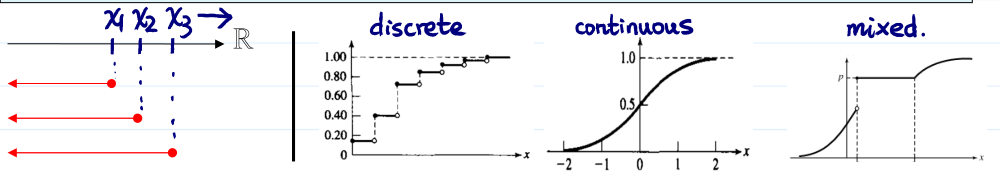
\includegraphics[width=0.8\textwidth]{image/cdf.png}
\end{figure}

\begin{definition}[概率质量函数]
    当$\mathcal{X}$是(至多可数的)离散点集, 设$\mathscr{F}_{\mathcal{X}}$由$\mathcal{X}$的所有子集组成, 此时$X$的分布由\textbf{概率质量函数}(probability mass function, p.m.f.)
    \[ p_{X}(x) = \P\{X=x\} = \P(\{\omega\in\Omega:X(\omega)=x\}), \quad x\in\mathcal{X} \]
    唯一刻画.
\end{definition}

\begin{remark}
    这是概率的哪个性质保证的?
\end{remark}

\begin{definition}
    当$\mathcal{X} = \R^{n}$, 考虑$\mathscr{F}_{\mathcal{X}}$为$\left\{\prod_{i=1}^{n}(-\infty,x_{i}] : x_{1},\dots,x_{n}\in\R\right\}$生成的Borel代数(最小的$\sigma$代数), 此时$X = (X_{1},\dots,X_{n})^{\top}$的分布由(累积)\textbf{分布函数}(cumulative distribution function, c.d.f.)
    \[ F_{X}(x_{1},\dots,x_{n}) = \P\{X_{1}\leq x_{1},\dots, X_{n}\leq x_{n}\}, \quad x_{1},\dots,x_{n}\in\R. \]
    唯一刻画. 若$F_{X} : \R^{n} \to [0,1]$可微(或者更一般地, \emph{绝对连续}), 称
    \[ f_{X} := \frac{\partial^{n} F_{X}}{\partial x_{1} \cdots \partial x_{n}} \]
    为$X$的\textbf{概率密度函数}(probability density function, p.d.f.), 此时称$X$为\textbf{连续型随机向量}.
\end{definition}

\section{随机变量的条件分布}

记$\sigma(X) := X^{-1}(\mathscr{F}_{\mathcal{X}}) := \{X^{-1}(B):B\in\mathscr{F}_{\mathcal{X}}\}$. 根据前面的定义, $X$可测当且仅当$\sigma(X) \subset \mathscr{F}$. 若随机元$X_{1} : (\Omega,\mathscr{F}) \to (\mathcal{X}_{1},\mathscr{F}_{\mathcal{X}_{1}})$与随机元$X_{2} : (\Omega,\mathscr{F}) \to (\mathcal{X}_{2},\mathscr{F}_{\mathcal{X}_{2}})$满足$\sigma(X_{1})\indep\sigma(X_{2})$, 则称$X_{1}$与$X_{2}$\textbf{独立}, 记为$X_{1} \indep X_{2}$.

\emph{注}: 对任意\emph{可测}映射$g_{1},g_{2}$成立$X_{1} \indep X_{2} \implies g_{1}(X_{1}) \indep g_{2}(X_{2})$. 事实上, $\sigma(g(X)) \subset \sigma(X)$.

当$X_{1}$和$X_{2}$都是实值随机向量时, $X_{1} \indep X_{2}$当且仅当(\emph{思考}: $\sigma(X^{-1}(\bullet)) = X^{-1}(\sigma(\bullet)), \ \bullet\subset\mathscr{F}_{\mathcal{X}}$?)
\[ F_{X_{1},X_{2}}(x_{1},x_{2}) = F_{X_{1}}(x_{1})F_{X_{2}}(x_{2}), \ \forall x_{1},x_{2}. \]
对于连续型随机向量, 刻画独立性只需要
\[ f_{X_{1},X_{2}}(x_{1},x_{2}) = f_{X_{1}}(x_{1})f_{X_{2}}(x_{2}), \ \forall x_{1},x_{2}. \]

设随机向量$X$和$Y$有\emph{联合}(joint)概率密度函数$f_{X,Y}$, 可以证明$X$有概率密度函数
\[ f_{X}(\cdot) = \int f_{X,Y}(\cdot,y) \,\d{y}, \] 称为$(X,Y)$中$X$的\emph{边际}(margin)概率密度函数. \textbf{$Y$条件于$X=x$的概率密度函数}$f_{Y|X}(\cdot|x)$满足
\[ f_{X,Y}(x,\cdot) = f_{Y|X}(\cdot|x)f_{X}(x). \]

\section{随机变量的函数}

